\documentclass[12pt,onecolumn,a4paper]{report}

\usepackage{mathtools}
\usepackage[top=60pt,bottom=60pt,left=50pt, right=50pt]{geometry}
\usepackage{graphicx}
\usepackage{wrapfig}
\usepackage{caption}
\usepackage{subcaption}
\usepackage{listings}

\graphicspath{{../plots/}}
\renewcommand*\thesection{\arabic{section}}

\newfont{\pica}{cmpica scaled 800}

\begin{document}
\title{COMP3032 Assignment: Image Contour Extraction}
\author{ \textbf{ Dionisio Perez-Mavrogenis}\\
		School of Electronics and Computer Science \\
		Faculty of Physical and Applied Sciences \\
		University of Southampton}
\maketitle

\tableofcontents
\pagebreak

\section{Introduction}
\subsection{Equations used}

The equations used for extracting the optimal contour from the provided image were the following :
\begin{equation}
E(v) = \sum^{N-2}_{i=1} E_i (v_{i-1},v_i,v_{i+1})
\end{equation}

\begin{equation}
E_i (v_{i-1},v_i,v_{i+1}) = \lambda \frac{|v_{i+1} - 2v_i + v_{i+1}|^2}{|v_{i+1} - v_{i-1}|^2} + (1-\lambda)I(v_i)
\end{equation}

\begin{equation}
S_i(v_{i+1},v_i) = \min_{v_{i-1}}[S_{i-1}(v_i,v_{i-1}) + E_i (v_{i-1},v_i,v_{i+1})]
\end{equation}

\begin{equation}
E(v_i) = \lambda |v_i - v_{i-1}| + (1-\lambda)I(v_i)
\end{equation}

\begin{equation}
S_i(v_i) = \min_{v_{i-1}}[S_{i-1}(v_{i-1})+E_i(v_{i-1},v_i)]
\end{equation}

where $\lambda \in [0,1]$ is the regularization parameter and $S_0(v_1,v_0) = 0$.
\section{Approach}
The coursework was coded in Matlab. Although the approach I have chosen is not exactly the same as the one in the specification(with differences highlighted as encountered), my implementation works fairly well.
The image used was the file "tongue.png" provided with the specification, but the images displayed in the report are zoomed-in in the area enclosed be the contours because it is easier to spot details.
\subsection{Constructing the search space}
The construction of the search space is done by the function {\pica get\_search\_space}. Given a number $M$, the search space created will have $M*N$ points, where $M$ includes both points on the starting contours(only $M-2$ points are created). 

The search space is constructed in the following manner : 
for each point in the first contour, calculate the $x$ and $y$ difference with the corresponding point in the second contour ($ xdif_i = abs[v_{i,1}(x) - v_{i,2}(x)]/(M-1),ydif_i = abs[v_{i,1}(y) - v_{i,2}(y)]/(M-1) $) and then to get each new point $v'(i)$ between points $v_{i,1},v_{i,2}$ do :

\begin{displaymath}
v'_i = [xdif_i*(J-1)+v_{i,1}(x),ydif_i*(J-1)+v_{i,1}(y)], \forall J \in [1,M]
\end{displaymath}

where $v_{i,1}$ is point $i$ in contour $1$ and $dif_i$ is the absolute difference between points $(v_{i,1},v_{i,2})$(with $x$ and $y$ denoting the corresponding coordinate).I add $dif*(J-1)$ to $v_{i,1}$ because contour one is assumed to be "bellow" contour two, that is, it has $x_1 \leq x_2$ and $y_1 \leq y_2$.
The {\pica get\_search\_space} function is given as inputs an M, the vector of contour1, the vector of contour2 and the matrix of intensities of the image and returns the intensity matrix for the search space points and matrices $X$ and $Y$, which contain the corresponding $x$ and $y$ coordinates of the search space points.
Because the results of calculating the search space point coordinates might not always yield an integer, Matlab's inbuilt function {\pica round} function was used.

The code for {\pica get\_search\_space} is given in Appendix A 0.1, Listing A.2, and samples of the generated search space are shown in Appendix B 0.3, Figure B.1 . 

\subsection{Construction of Energy and Position matrices}

The function {\pica get\_matrices} is responsible for calculating the energy and position matrices. It is supplied with arguments : $\lambda$ (the regularization parameter), the intensity matrix calculated by {\pica get\_search\_space}, and the $X$ and $Y$ matrices(also calculated by {\pica get\_search\_space}), and returns the energy matrix (an $M\times N\times M$ matrix) and a vector describing which points belong to the optimal contour (the backtracking is also done in this function), which then is handled by the plotting functions who locate the actual points on the image later on.

For a given point $v_i$ , the entry in the energy matrix is calculated according to equation(3), with resulting value being inserted in $en(y,x,z)$ and $z$ being equal to the $y$ index of $v_{i+1}$. The energy up to point $v_i$ is taken to be the energy between points $v_{i-1}$ and $v_i$, as this is assumed to be the optimal between these two and thus the optimal between the triplet.

Simultaneously, the position matrix is being built. At each position, $posm(y,x,z)= z' $, where $z'$ is the $y$-index of the optimal $v_{i-1}$ point and $z$ represents the $y$-index of the $v_{i+1}$ point for which this calculation is taking place.

The first and last columns of the position and energy matrices present a special case, since we need points $v_0$ and $v_{N+1}$ to calculate results for points in columns 1 and N, and such points do not exist. Therefore, column 1 is initialized to 0,  and the energy for points in column N is calculated by equations (4) and (5).

Backtracking involved searching through the N-1 column of the energy matrix for the row that contained the minimum value , record the position of the row($y$-index) and the position of the minimum value in the row($z$-index). The rest of the procedure involves setting $y=z$ and reading $posm(y,x,z)$ into  $z$, then repeating the process for every $x \in [2,N-1]$.

The code for this section is given in Appendix A, Listing A.3. The plotting functions are called in the invoking script, which is given in Appendix A, Listing A.1.

\section{Evaluation of the algorithm}
The evaluation following is not general and refers only to my implementation. Also, timings were performed using Matlab's {\pica tic toc} function, on machines in the Zepler labs.

\subsection{Robustness}
\paragraph{Robustness to different initialisations }


\begin{figure}[Ht]
        \centering
        \begin{subfigure}[b]{0.45\textwidth}
                \centering
                \includegraphics[width=\textwidth]{3D/{clcap-100-0.05000}.png}
                \caption{Initialized to 0.}
        \end{subfigure}%
        ~ %add desired spacing between images, e. g. ~, \quad, \qquad etc. 
          %(or a blank line to force the subfigure onto a new line)
        \begin{subfigure}[b]{0.45\textwidth}
                \centering
                \includegraphics[width=\textwidth]{3D/{clcapnz-100-0.05000}.png}
                \caption{Initialized to intensity.}
        \end{subfigure}
        \caption{Optimal contour for different initialization of the energy matrix(M=100,$\lambda=0.05$.)}
\end{figure}

Two different initialization methods were tried to test the algorithms robustness. The first method set the energies of the first column to zero, as the coursework suggested, whereas the second set each point's energy to be equal to its intensity.

Figure 1 displays the resulting optimal contour for different initializations. The algorithm is robust enough so that the only difference is not on the actual contour being traced, but on the black space to the left of the tongue. Once the algorithm finds the optimal contour, the two contours are effectively identical.



\paragraph{Robustness for varying values of $\lambda$}
With an initial value of $\lambda=0.5$ the results were not satisfactory,as the result of tracing deviated a lot from the desired result, whereas when varying $\lambda$ it was found that acceptable results are obtained when $\lambda < 0.2$, and improved as $\lambda$ got smaller. 

\begin{figure}[Ht]
        \centering
        \begin{subfigure}[b]{0.45\textwidth}
                \centering
                \includegraphics[width=\textwidth]{3D/{clcap-100-0.05000}.png}
                \caption{$\lambda=0.05$}
        \end{subfigure}%
        ~ %add desired spacing between images, e. g. ~, \quad, \qquad etc. 
          %(or a blank line to force the subfigure onto a new line)
        \begin{subfigure}[b]{0.45\textwidth}
                \centering
                \includegraphics[width=\textwidth]{3D/{clcap-100-0.50000}.png}
                \caption{$\lambda=0.5$}
        \end{subfigure}
        \caption{Optimal contour for different values of $\lambda$(M=100)}
\end{figure}

Figure 2 shows a comparison for different $\lambda$ values and Appendix B 0.4 shows resulting traces for for different values of $\lambda$


\subsection{Performance}

\begin{figure}[Htb]
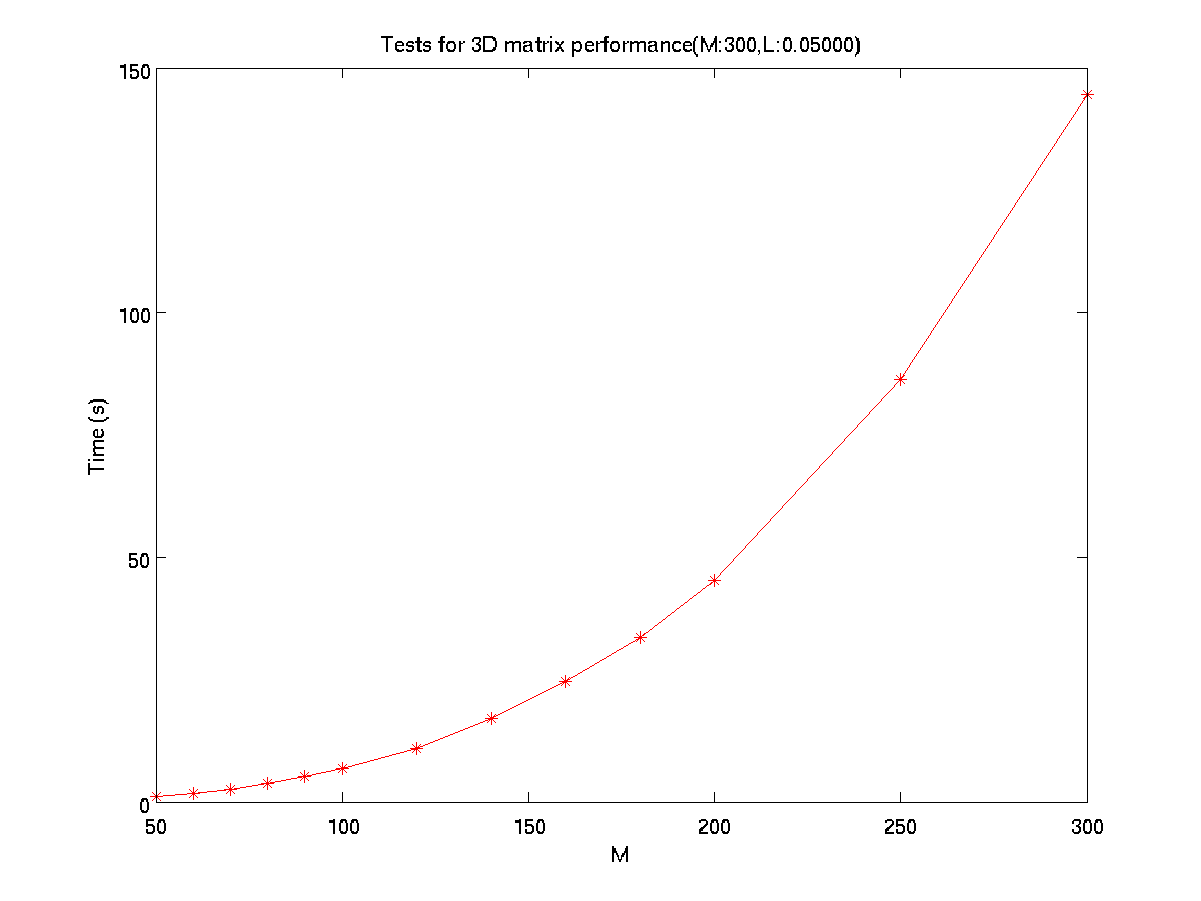
\includegraphics[scale=0.5]{3D/cw_3d_benchmark.png}
\centering
\caption{Benchmark of 3D matrix implementation for various values of M.}
\end{figure}

This algorithm performs for $N-1$ columns(where $N$ is the number of points in the initial contours), for $M$ points, $M\times M$ operations and thus a good approximation for the running time would be $N\times M^3$, and one hypothesis suggests that the algorithms has $O(M^3)$ running time, since N could be considered a constant. My implementation uses four {\pica for}-loops to perform the calculations and all calculations have been moved to the outermost loop possible .

Figure 3 is plot of the value of $M$ and the corresponding running times. The shape of the curve suggests an exponential function for the total running time. It has been observed that changing the value of $\lambda$ has no impact on the running time for any given $M$.

\subsection{Application to other images}

\begin{figure}[Ht]
        \centering
        \begin{subfigure}[b]{0.5\textwidth}
                \centering
                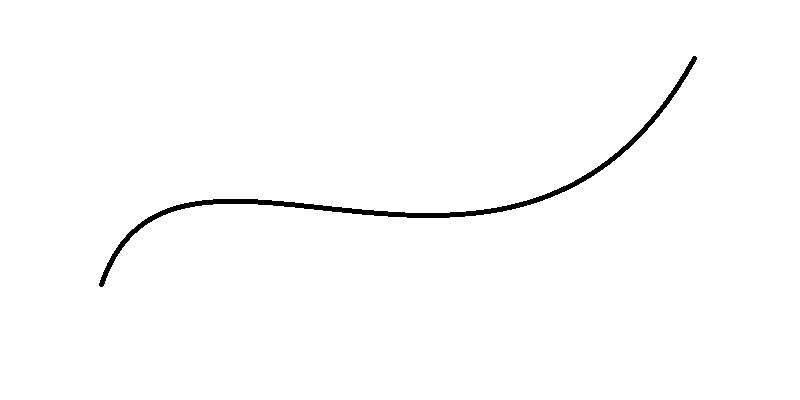
\includegraphics[width=\textwidth]{curve.png}
                \caption{The random curve}
        \end{subfigure}%
        ~ %add desired spacing between images, e. g. ~, \quad, \qquad etc. 
          %(or a blank line to force the subfigure onto a new line)
        \begin{subfigure}[b]{0.5\textwidth}
                \centering
                \includegraphics[width=\textwidth]{3D/{curvez-150-0.05000}.png}
                \caption{The traced contour.}
        \end{subfigure}
        \caption{Application to a random curve(M=150)}
\end{figure}
The algorithm was applied to the image of a curve that I created, and the results are shown in Figure 4.
The result shown in Figure 4(b) is for M=150,$\lambda$=0.05 and a zero initialization of the energy matrix's first column. 
There is a small part in the beginning of the curve that is not tracked (missing points from the initial contours), and the two initial points of the optimal contour that are completely off the curve, as well as the last point of the tracing. These might be attributed to the initialization of the energy matrix's first column and different calculation for the last column's energy. However, when the algorithm "finds" the black curve it tracks the curve correctly, confirming that the initial and last points pose a special case and could perhaps be ignored, or be dealt with in a different fashion.

\subsection{Comparison with a different algorithm}

\begin{figure}[Ht]
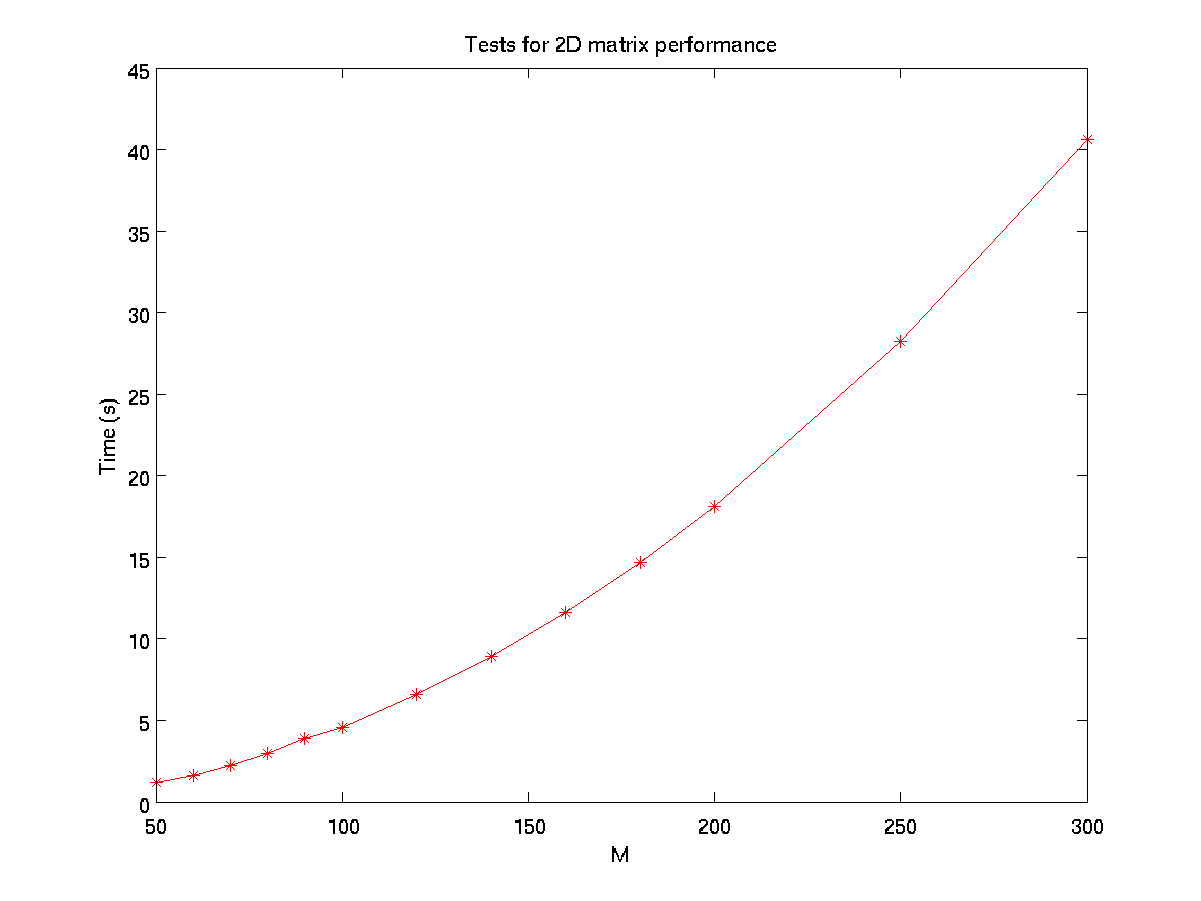
\includegraphics[scale=0.5]{2D/cw_2d_benchmark.png}
\centering
\caption{Benchmark of 2D matrix implementation for various values of M.}
\end{figure}

\begin{figure}[Ht]
        \centering
        \begin{subfigure}[b]{0.5\textwidth}
                \centering
                \includegraphics[width=\textwidth]{3D/{clcap-100-0.05000}.png}
                \caption{3D matrix, M=100,$\lambda=0.05$}
        \end{subfigure}%
        \begin{subfigure}[b]{0.5\textwidth}
                \centering
                \includegraphics[width=\textwidth]{2D/{2d-clcap-100-0.05000}.png}
                \caption{2D matrix, M=100,$\lambda=0.05$}
        \end{subfigure}
        
        \begin{subfigure}[b]{0.5\textwidth}
                \centering
                \includegraphics[width=\textwidth]{3D/{clcap-300-0.05000}.png}
                \caption{3D matrix, M=300,$\lambda=0.05$.}
        \end{subfigure}
        
        \begin{subfigure}[b]{0.5\textwidth}
                \centering
                \includegraphics[width=\textwidth]{2D/{2d-clcap-300-0.05000}.png}
                \caption{2D matrix, M=300,$\lambda=0.05$.}
        \end{subfigure}
        \caption{Comparison of the two algorithms}
\end{figure}


\begin{figure}[Ht]
\includegraphics[scale=1]{2D/{2d-curve-150-0.00500}.png}
\centering
\caption{Tracing of curve by 2D algorithm ($M=150,\lambda=0.005$), with portions of the contour being completely straight, illustrating this algorithm's linear sense of continuity.}
\end{figure}


A second algorithm was implemented in order to extract the contour of the tongue. This is the algorithm presented in the "Dynamic Programming" lecture, and uses Equations (4) and (5) to extract the optimal contour. The algorithm performs a total of $N\times M\times M$ operations; a benchmark of this algorithm's performance is given in Figure 5, and its time complexity could be characterized as $O(M^2)$, if we treat $N$ as a constant term.

Figure 6 shows a comparison of the contours extracted from the two algorithms. Both algorithms extracted the optimal contour fairly well, the 2D implementation being simpler and faster to implement and seems to extract a smoother contour. However, the 2D algorithm has got a sense of continuity that approximates a straight line because it only considers two points, something that is illustrated in Figure 7.

Code for this algorithm is given in Appendix A.2.

\section{Conclusion}
This implementation of the algorithm might not be the optimal, as I am not as proficient in Matlab, however it illustrates that the algorithm works and allows comparison with other algorithms.
Also, even though the background of the image containing the tongue is the original one, the algorithms run on the negated version of that image (so that the contour we extract has the minimum energy) and the result is plotted on the original image.

%

%		APPENDICES 

%


\pagebreak
\appendix
\chapter{Code listings}
\subsection{Code for the 3D matrix algorithm}

\lstset{ %
  language=Matlab,                % the language of the code
  numbers=left, 
  caption={Code used to initialize, run and plot the results for the 3D algorithm.},
}
\lstinputlisting{../start_coursework_3D.m}

\lstset{ %
  language=Matlab,                % the language of the code
  numbers=left, 
  caption={Function generating the search space for the 3D algorithm.},
}
\lstinputlisting{../get_search_space.m}

\lstset{
  language=Matlab,
  numbers=left, 
  caption={Function generating the position and energy matrices and doing the backtracking.},
}
\lstinputlisting{../get_matrices_3D.m}

\lstset{
  language=Matlab,
  numbers=left, 
  caption={Function that gets the optimal points returned from {\pica get\_matrices} and retrieves their (x,y) coordinates, and adds them to an $N\times 2$ vector for the plotting functions.},
}
\lstinputlisting{../get_optimals_3D.m}

\subsection{Energy extraction function of 2D matrix.}
Since the search space extraction and plotting functions are identical to the 3D implementation, only the energy calculation and back-tracking code for the 2D implementations is shown.
\lstset{
  language=Matlab,
  numbers=left, 
  caption={Function that generates the position and energy matrices for the 2D implementation of the algorithm.},
}
\lstinputlisting{../2D_implementation/fill_energy_matrix.m}

\lstset{
  language=Matlab,
  numbers=left, 
  caption={Function that does the calculation for the transition between points $v_{i-1},v_i$.},
}
\lstinputlisting{../2D_implementation/point_energy.m}

\chapter{Some of the images generated}

\subsection{Images of the search space generated}
These are two sample images generated by the {\pica get\_search\_space} function. The search points are not plotted together with the optimal contour because the resulting image would get too cluttered to draw any results.
\begin{figure}[ht]
        \centering
        \begin{subfigure}[b]{0.5\textwidth}
                \centering
                \includegraphics[width=\textwidth]{3D/{sspace-50}.png}
                \caption{Search space generated for M=50}
        \end{subfigure}%
        \begin{subfigure}[b]{0.5\textwidth}
                \centering
                \includegraphics[width=\textwidth]{3D/{sspace-50}.png}
                \caption{Search space generated for M=100}
        \end{subfigure}
        \caption{Plotting of two sample search spaces.}
\end{figure}

\subsection{Traced contours for different values of $\lambda$}
\begin{figure}[H]
\centering
        \begin{subfigure}[b]{0.5\textwidth}
                \centering
                \includegraphics[width=\textwidth]{3D/{100-0.05000}.png}
                \caption{$\lambda=0.05$}
        \end{subfigure}%
        \begin{subfigure}[b]{0.5\textwidth}
                \centering
                \includegraphics[width=\textwidth]{3D/{100-0.15000}.png}
                \caption{$\lambda=0.15$}
        \end{subfigure}
        \begin{subfigure}[b]{0.5\textwidth}
	        	\centering
    		    \includegraphics[width=\textwidth]{3D/{100-0.30000}.png}
	        	\caption{$\lambda=0.3$}
        \end{subfigure}
        \begin{subfigure}[b]{0.5\textwidth}
                \centering
                \includegraphics[width=\textwidth]{3D/{100-0.50000}.png}
                \caption{$\lambda=0.5$}
        \end{subfigure}
        \caption{Plotting of two sample search spaces, with M=100.}
\end{figure}

These tracings are generated by the 3D energy matrix algorithm and have $M=100$.
\end{document}